
\chapter{相关性、关联性及尤尔-辛普森悖论}
 \label{chapter::correlationassociation}
 
 
因果关系是人类知识的核心。以下为古希腊的两条著名名言。 


\begin{quote}
“我宁愿发现一条因果定律，也不愿成为波斯国王。”

--- 德谟克利特 
\end{quote}


\begin{quote}
“在弄清事物的原因之前，我们不可能真正了解它。”

--- 亚里士多德 
\end{quote}
 
 
然而，传统统计学的主要内容是研究变量间的关联性而非因果关系。本章将回顾一些基本的关联性度量方法，并指出它们存在的根本性局限。 
 

\section{统计学的传统观点}

统计学的传统观点是推断变量之间的相关性或关联性。基于这种观点，统计学中不存在因果推断的必要。与该观点相关的两条著名格言如下：

\begin{itemize}
\item
“相关性并不意味着因果关系。”

\item
“无法通过统计学证明因果关系。” 
\end{itemize}

本书的观点则大相径庭：统计学对于理解因果关系至关重要。本书的核心目标是介绍因果推断的形式化语言，并开发用于随机实验与观察性研究中估计因果效应的统计方法。 




 
\section{常用的关联性度量方法}


\subsection{相关性与回归}
\label{section:correlatioandregressionintro}

随机变量$Z$与$Y$之间的 Pearson 相关系数为
$$
\rho_{ZY} = \frac{  \cov(Z, Y)   }{   \sqrt{   \var(Z) \var(Y)   }   } ,
$$
它衡量$Z$与$Y.$之间的线性依赖程度。
 

以 $Z$ 为自变量、$Y$ 为因变量的线性回归模型为 
\begin{equation}
Y = \alpha + \beta Z + \varepsilon ,
\label{eq::short-regression}
\end{equation} 
其中 $E(   \varepsilon  ) = 0$ 且 $E(   \varepsilon  Z ) = 0 $。可以证明回归系数 $\beta$ 满足  
 $$
 \beta = \frac{  \cov(Z, Y)   }{   \var(Z)    }  = \rho_{ZY}   \sqrt{     \frac{  \var(Y)     }{ \var(Z)  }    }  . 
 %\propto \rho_{XY}  .
 $$
 因此 $\beta$ 与 $\rho_{ZY} $ 的符号始终相同。 
 
 
也可定义$Y$对$Z$和$X$的多元回归：
\begin{equation}
 Y = \alpha  + \beta Z + \gamma  X + \varepsilon ,
 \label{eq::long-regression}
\end{equation}
其中$E( \varepsilon) = 0, E( \varepsilon Z) = 0$且$ E( \varepsilon X) = 0$。通常将$\beta$解释为$Z$对$Y$的“效应”，并称为{\it 固定$X$}、{\it 以$X$为条件}或{\it 控制$X$}后的效应。第\ref{appendix::basic-linear-regression}章回顾线性回归的基础。 

 

更有意思的是，回归式\eqref{eq::short-regression}和\eqref{eq::long-regression}中的$\beta$可能不同，甚至符号相反。下面的\ri{R}代码重新分析\citet{hainmueller2012entropy}使用的 LaLonde 观察性数据，研究职业培训对收入的“因果效应”。控制全部协变量后，\ri{treat}的系数为\ri{1067.5461}；不控制任何协变量时，\ri{treat}的系数为\ri{-8506.4954}。 


\begin{lstlisting}
> dat <- read.table("cps1re74.csv", header = TRUE)
> dat$u74 <- as.numeric(dat$re74==0)
> dat$u75 <- as.numeric(dat$re75==0)
> 
> ## linear regression on the outcome
> ## . means regression on all other variable in dat
> lmoutcome = lm(re78 ~ ., data = dat)
> round(summary(lmoutcome)$coef[2, ], 3)
  Estimate Std. Error    t value   Pr(>|t|) 
  1067.546    554.060      1.927      0.054 
> 
> lmoutcome = lm(re78 ~ treat, data = dat)
> round(summary(lmoutcome)$coef[2, ], 3)
  Estimate Std. Error    t value   Pr(>|t|) 
 -8506.495    712.766    -11.934      0.000 
\end{lstlisting} 



 
 
 \subsection{列联表}
 \label{sec::twobytwotables-withresume}
 
 我们可以用一个二乘二列联表来表示两个二元变量 $Z$ 与 $Y$ 的联合分布。设 $p_{zy} = \pr( Z=z, Y=y )$，则联合分布可表示为下表：
 
 
 \begin{center}
\begin{tabular}{lcc}
\hline 
        & $Y =1$ & $Y =0$\\\hline
$Z =1$ & $p_{11}$ & $p_{10}$\\ 
$Z =0$ & $p_{01}$ & $p_{00}$\\ 
\hline 
\end{tabular}
\end{center}
 
 
 若将 $Z$ 视为干预措施、$Y$ 视为结果变量，则可定义风险差（Risk Difference）为
\begin{eqnarray*}
\RD  &=& \pr(Y=1\mid Z=1) - \pr(Y=1\mid Z=0)  \\
&=& \frac{p_{11}}{ p_{11} + p_{10} } -  \frac{p_{01}}{ p_{01} + p_{00} } ,
\end{eqnarray*}
风险比（Risk Ratio）为
\begin{eqnarray*}
 \RR &=&  \frac{ \pr(Y=1\mid Z=1)  }{    \pr(Y=1\mid Z=0)    }  \\
& =&   \frac{p_{11}}{ p_{11} + p_{10} }  \Big /  \frac{p_{01}}{ p_{01} + p_{00} } ,
\end{eqnarray*}
优势比（Odds Ratio）\footnote{在概率论中，某一事件的比值定义为该事件发生概率与不发生概率之比。}为
\begin{eqnarray*}
 \OR &=& \frac{ \pr(Y=1\mid Z=1) /  \pr(Y=0\mid Z=1)  }{    \pr(Y=1\mid Z=0) /\pr(Y=0\mid Z=0)   }  \\
& =& \frac{      \frac{p_{11}}{ p_{11} + p_{10} } /  \frac{p_{10}}{ p_{11} + p_{10} }  }{  \frac{p_{01}}{ p_{01} + p_{00} } / \frac{p_{00}}{ p_{01} + p_{00} }     }  \\
 &=& \frac{ p_{11} p_{00}  }{  p_{10} p_{01} }.
\end{eqnarray*}

“风险差”、“风险比”和“优势比”这些术语源于流行病学。由于流行病学研究的对象多为疾病，因此用“风险”来描述患病概率十分自然。 
 
 
关于这些度量指标有以下基本结论：
\begin{proposition}\label{prop::2x2-independence}
(1) 以下命题均等价\footnote{本书使用符号 $\ind$ 表示随机变量的独立性或条件独立性，该符号由 \citet{dawid1979conditional} 提出。}：$Z\ind Y $, $\RD = 0$、$\RR = 1$ 以及 $\OR = 1$。 
(2) 若所有 $p_{zy}$ 值均大于零，则 $\RD >0$ 等价于 $\RR >1$，也等价于 $\OR > 1$。 
(3)
当 $\pr(Y=1\mid Z=1)$ 与 $ \pr(Y=1\mid Z=0)$ 取值较小时，$\OR \approx \RR$。 
\end{proposition}

命题 (1) 与 (2) 的证明留作习题\ref{hw::2x2-equivalence}。命题 (3) 是非正式近似：对罕见疾病，$p\approx 0$，优势$p/(1-p)$接近概率$p$，因为 Taylor 展开给出$p/(1-p) = p + p^2 + \cdots\approx p $。流行病学结果为罕见疾病时，假定$\pr(Y=1\mid X=1)$与$ \pr(Y=1\mid X=0)$较小是合理的。 
 

 
还可定义以下度量的条件版本： \textsc{rd}、 \textsc{rr}和 \textsc{or}，只需将概率替换为给定另一变量$X$后的条件概率，即$\pr(Y=1\mid Z=1, X=x) $与$ \pr(Y=1\mid Z=0, X=x)  .$。
 
 
设观测样本中符合各分类的观测值数目为 $n_{zy} = \#\{i:  Z_i=z, Y_i=y \}$，则可构建如下二乘二列联表来汇总数据：
 \begin{center}
\begin{tabular}{lcc}
\hline 
        & $Y =1$ & $Y =0$\\\hline
$Z =1$ & $n_{11}$ & $n_{10}$\\ 
$Z =0$ & $n_{01}$ & $n_{00}$\\ 
\hline 
\end{tabular}
\end{center}
可以估计  \textsc{rd}、 \textsc{rr}和 \textsc{or}，计算时以样本比例$\hat p_{zy} = n_{zy}  / n$替代真实概率，$n$为总样本量（见第\ref{section::asymptotic-inference-2x2}节）。在\ri{R}中，可根据观测数据的二乘二表，用\ri{fisher.test}对$Z \ind Y$作精确检验，或用\ri{chisq.test}作渐近检验。 
 
 
 \begin{example}\label{eg::bertrand2004emily-chapter1}
 \citet{bertrand2004emily} 开展了一项基于简历的随机实验，旨在研究感知种族因素对求职回音率的影响。实验要求作者们将虚构的求职简历分别署上听感像黑人或白人的名字，再投递至波士顿与芝加哥的报纸征才广告中。以下为描述感知种族与回音情况的二乘二列联表：
 
 \begin{lstlisting} 
> resume = read.csv("resume.csv")
> Alltable = table(resume$race, resume$call)
> Alltable
       
           0    1
  black 2278  157
  white 2200  235
    \end{lstlisting} 


由于表格中两行的总数相同，可见署上白人名字的简历获得回音的频率更高。随后的费舍尔精确检验证明这种差异具有统计学显著性。    
     \begin{lstlisting} 
> fisher.test(Alltable)

	Fisher's Exact Test for Count Data

data:  Alltable
p-value = 4.759e-05
alternative hypothesis: true odds ratio is not equal to 1
95 percent confidence interval:
 1.249828 1.925573
sample estimates:
odds ratio 
  1.549732 
  \end{lstlisting} 
 
 \end{example}
 
\section{尤尔-辛普森悖论实例} 

\subsection{数据来源}
该肾结石研究实例引自 \citet{charig1986comparison}。在该研究中，$Z$ 为干预措施变量，取值 $1$ 代表开放式手术，$0$ 代表微创穿刺术；$Y$ 为结果变量，取值 $1$ 表示治疗成功，$0$ 表示治疗失败。相关数据可汇总为如下二乘二列联表： 

 \begin{center}
\begin{tabular}{lcc}
\hline 
        & $Y =1$ & $Y =0$\\\hline
$Z =1$ & $273$ & $77$\\ 
$Z =0$ & $289$ & $61$\\ 
\hline 
\end{tabular}
\end{center}



估计的 \textsc{rd}为
$$
\widehat{\RD} = \frac{273}{273 + 77} - \frac{289}{289 + 61} = 78\% - 83\% = -5\% <0. 
$$
处理 0 看起来更好，即小切口穿刺术比开放手术有更高的成功率。 


然而，该数据并非源自随机对照试验（RCT）\footnote{在随机对照试验中，患者被随机分配至不同干预组。本书 \ref{part::rcts} 部分将专门探讨此类研究。}。接受干预措施 $1$ 的患者群体特征与接受干预措施 $0$ 的患者群体特征存在显著差异。此处存在一个重要混淆变量：病情严重程度。部分患者结石较小，部分患者结石较大。我们可以按结石尺寸对患者进行分类。 


对于结石较小的患者群体，相关数据可汇总为如下表格： 
 \begin{center}
\begin{tabular}{lcc}
\hline 
        & $Y =1$ & $Y =0$\\\hline
$Z =1$ & $81$ & $6$\\ 
$Z =0$ & $234$ & $36$\\
\hline 
\end{tabular}
\end{center}
对较大结石患者，处理与结果可汇总为以下二乘二表：  
 \begin{center}
\begin{tabular}{lcc}
\hline 
        & $Y =1$ & $Y =0$\\\hline
$Z =1$ & $192$ & $71$\\ 
$Z =0$ & $55$ & $25$\\
\hline 
\end{tabular}
\end{center}


后两个表的计数加起来必须等于第一个表：
$$
81 + 192 = 273,\quad 6 + 71 =77,\quad   234 + 55 = 289, \quad 36 + 25 = 61 .  
$$
在较小结石患者中，估计的 \textsc{rd}为
$$
\widehat{\RD}_\text{smaller} = \frac{81}{81 + 6} - \frac{234}{234 + 36} = 93\% - 87\% = 6\% > 0,
$$
表明处理 1 更好。在较大结石患者中，估计的 \textsc{rd}为
$$
\widehat{\RD}_\text{larger} = \frac{192}{192 + 71} - \frac{55}{55+25} = 73\% - 69\% = 4\% > 0 ,
$$
同样表明处理 1 更好。 


上述分析得到
$$
\widehat{\RD} < 0,\quad
\widehat{\RD}_\text{smaller} >0, \quad
\widehat{\RD}_\text{larger}  > 0 .
$$
非正式地说，处理 1 对小结石和大结石患者都更好，对全体患者却更差。若目标是推断处理效应，这种解释令人困惑。统计学称其为 Yule--Simpson 悖论或 Simpson 悖论：边际关联与所有水平上的条件关联符号相反。 




\subsection{现象解释}



令二元指标$X$取$X=1$表示小结石，$X=0$表示大结石。先比较两类患者接受处理 1 的概率，考察$X$与$Z$的关系：
\begin{eqnarray*}
&& \widehat{\pr}(Z=1 \mid  X=1) - \widehat{\pr}(Z=1 \mid X=0) \\
&=& \frac{81 + 6}{81 + 6 + 234 + 36} - \frac{192+71}{192 + 71 + 55 + 25} \\
&=&  24\% - 77\% \\
&=& - 53\% < 0 .
\end{eqnarray*}
大结石患者更常接受处理 1。统计上，$X$与$Z$负相关。 


再比较两类患者的成功概率，考察$X$与$Y$的关系。处理 1 下，
\begin{eqnarray*}
&& \widehat{\pr}(Y=1 \mid Z=1,  X=1) - \widehat{\pr}(Y=1 \mid Z=1,  X=0) \\
&=& \frac{81}{81 + 6} - \frac{192}{192 + 71} \\
&=& 93\% - 73\% \\
&=& 20\%
> 0;
\end{eqnarray*}
处理 0 下，
\begin{eqnarray*}
&& \widehat{\pr}(Y=1 \mid Z=0, X=1) - \widehat{\pr}(Y=1 \mid Z=0,   X=0) \\
&=& \frac{234}{234 + 36} - \frac{55}{55 + 25} \\
&=& 87\% - 69\% \\
&=& 18\% 
> 0.
\end{eqnarray*}
两种处理下，小结石患者的成功概率都更高。统计上，在任一处理水平下，$X$与$Y$均正相关。 


\begin{figure}
$$
\xymatrix{
 & X\ar_{-}[ld]\ar^{+}[rd] \\ 
Z \ar_{+}[rr] &&Y 
}
$$
\caption{肾结石例子的关系图。正负号表示两个变量之间的关联方向，条件是固定所有其他指向该下游变量的变量。}\label{fig::kidney-stone}
\end{figure}




图\ref{fig::kidney-stone}概括了这些定性关联。技术上，处理到结果既有正向路径$(Z\rightarrow Y)$，也有更强的负向路径$(Z\leftarrow X \rightarrow Y)$，所以处理与结果的总体关联为负。通俗地说，当效果较差的处理 0 更常用于病情较轻者时，它看起来反而可能更有效。 




一般而言，$X$与$Z$的关联以及$X$与$Y$的关联，会使$Z$与$Y$的边际关联，和给定$X$后$Z$与$Y$的条件关联在定性上不同。发生 Yule--Simpson 悖论时，称$X$为$Z$与$Y$关系的{\it 混杂变量}或{\it 混杂因素}，也说$Z$与$Y$受到$X$的{\it 混杂}。更深入讨论见第\ref{chapter::observational-studies}、\ref{chapter::evalue}章。 
 




\subsection{几何视角下的尤尔-辛普森悖论}


假设总体层面的数据汇总为如下二乘二表格：


 \begin{center}
\begin{tabular}{lcc}
\hline 
 全体样本       & $Y =1$ & $Y =0$\\\hline
$Z =1$ & $n_{11}$ & $n_{10}$\\ 
$Z =0$ & $n_{01}$ & $n_{00}$\\
\hline 
\end{tabular}
\end{center}


两个亚组的二乘二表计数为
 \begin{center}
\begin{tabular}{lcc}
\hline 
亚总体$X=1$        & $Y =1$ & $Y =0$\\\hline
$Z=1$ & $n_{11|1}$ & $n_{10|1}$\\ 
$Z=0$ & $n_{01|1}$ & $n_{00|1}$\\
\hline 
\end{tabular}
\end{center}
对应于$X=1$的亚组，以及
 \begin{center}
\begin{tabular}{lcc}
\hline 
亚总体$X=0$    & $Y =1$ & $Y =0$\\\hline
$Z =1$ & $n_{11|0}$ & $n_{10|0}$\\ 
$Z =0$ & $n_{01|0}$ & $n_{00|0}$\\
\hline 
\end{tabular}
\end{center}
对应于$X=0.$的亚组。


图\ref{fig::geomtry-simpson}展示 Yule--Simpson 悖论的几何解释。纵轴表示$Y=1$的成功数，横轴表示$Y=0$的失败数。两个平行四边形对应两个处理水平下成功和失败计数的合并。$OA_1$的斜率大于$OB_1$，$OA_0$的斜率大于$OB_0$，所以在$X$的两个水平内，处理似乎都有益。但$OA$的斜率小于$OB$，所以对整个总体，处理似乎有害，悖论由此产生。 





\begin{figure}
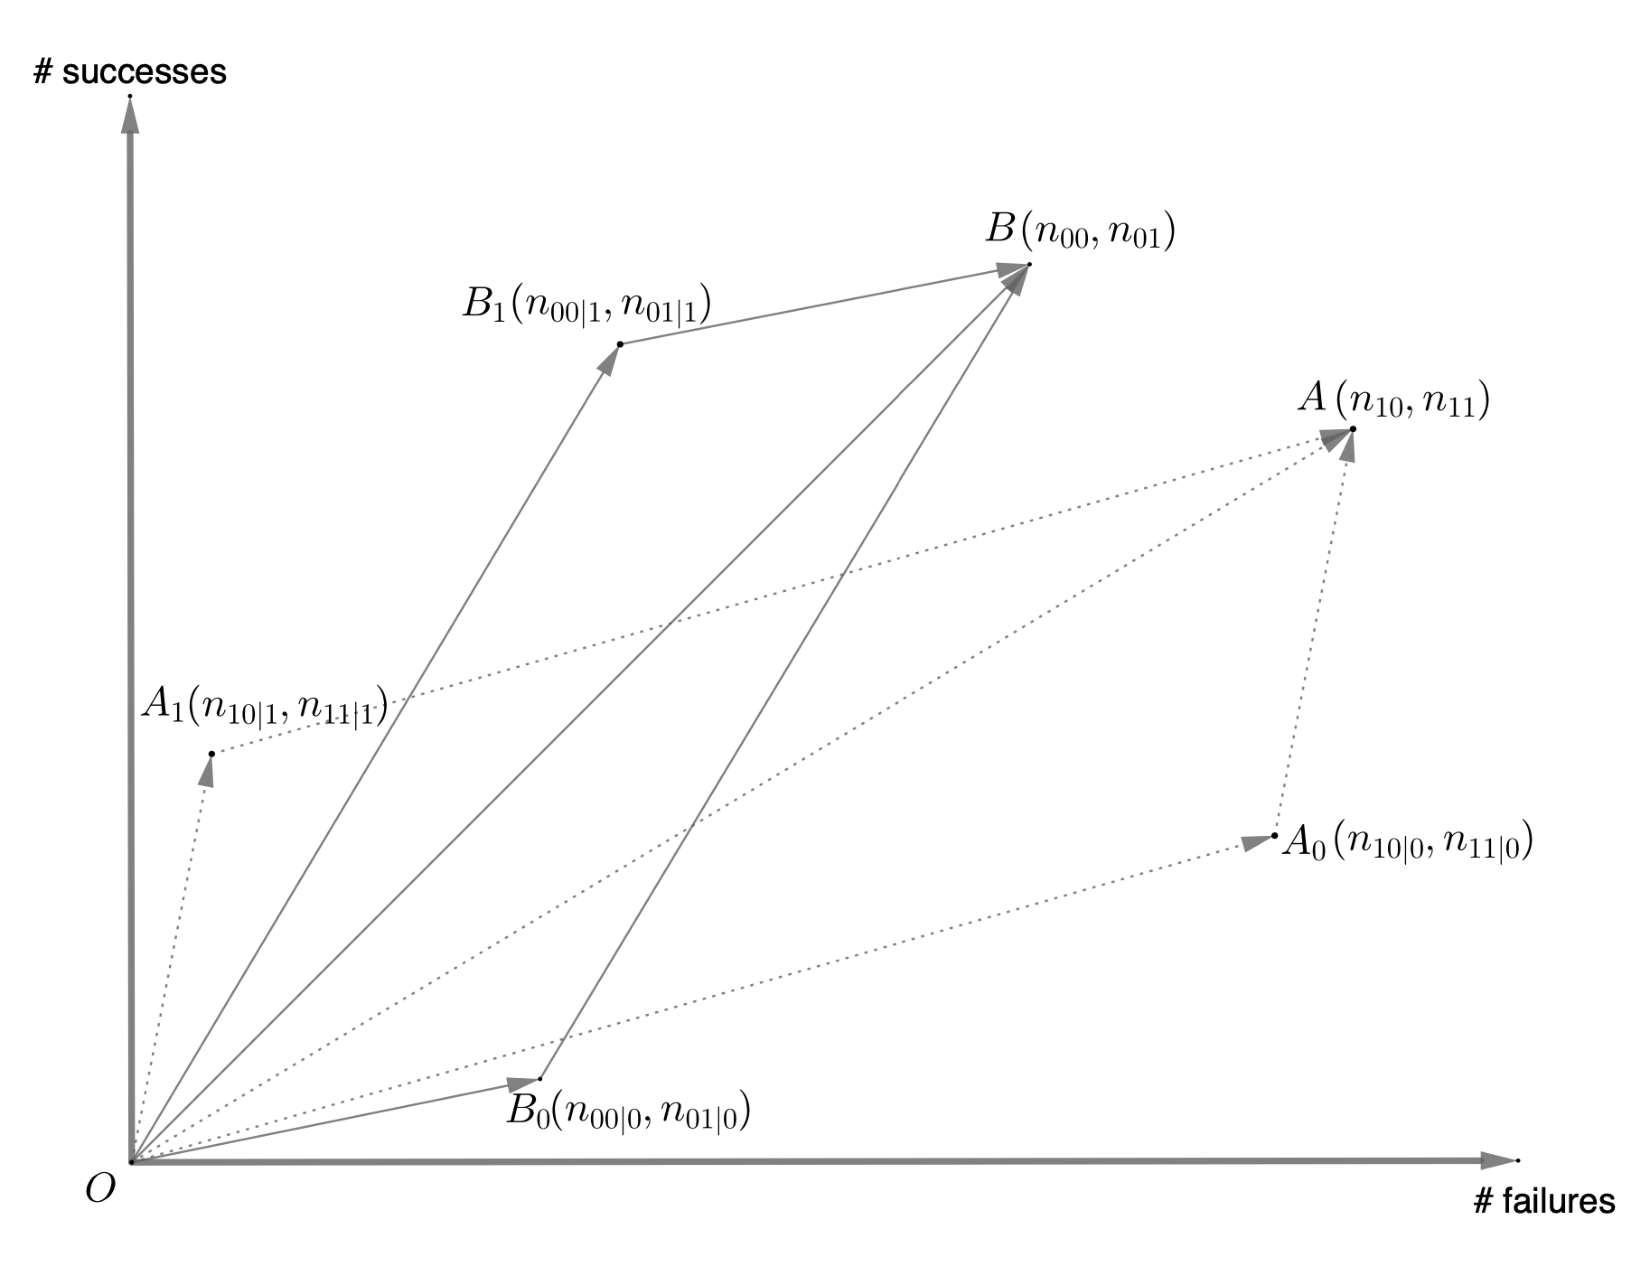
\includegraphics[width=\textwidth]{figures/simpson_geometry2.pdf}
\caption{尤尔-辛普森悖论的几何解释}\label{fig::geomtry-simpson}
\end{figure}

\section{伯克利大学研究生录取数据}
\label{sec::berkeleydata}

\citet{bickel1975sex} 曾研究伯克利大学研究生院的男女录取率差异。\ri{R} 语言的 \ri{datasets} 程序包中包含原始数据集 \ri{UCBAdmissions}。六个最大系别的原始数据如下所示： 
\begin{lstlisting}
> library(datasets)
> UCBAdmissions = aperm(UCBAdmissions, c(2, 1, 3))
> UCBAdmissions
, , Dept = A

        Admit
Gender   Admitted Rejected
  Male        512      313
  Female       89       19

, , Dept = B

        Admit
Gender   Admitted Rejected
  Male        353      207
  Female       17        8

, , Dept = C

        Admit
Gender   Admitted Rejected
  Male        120      205
  Female      202      391

, , Dept = D

        Admit
Gender   Admitted Rejected
  Male        138      279
  Female      131      244

, , Dept = E

        Admit
Gender   Admitted Rejected
  Male         53      138
  Female       94      299

, , Dept = F

        Admit
Gender   Admitted Rejected
  Male         22      351
  Female       24      317
\end{lstlisting}


对全系别数据汇总后可得简洁的二乘二列联表：
\begin{lstlisting} 
> UCBAdmissions.sum = apply(UCBAdmissions, c(1, 2), sum)
> UCBAdmissions.sum
        Admit
Gender   Admitted Rejected
  Male       1198     1493
  Female      557     1278
\end{lstlisting}

下面的函数以\ri{chisq.test}为基础，输入一个二乘二表，输出估计的 \textsc{rd}与$p$值：
\begin{lstlisting}
> risk.difference = function(tb2)
+ {
+   p1      = tb2[1, 1]/(tb2[1, 1] + tb2[1, 2])
+   p2      = tb2[2, 1]/(tb2[2, 1] + tb2[2, 2])
+   testp   = chisq.test(tb2)
+   
+   return(list(p.diff = p1 - p2,  
+               pv = testp$p.value))	    
+ }
\end{lstlisting}
运行该函数可知男女生的录取率存在显著差值：
\begin{lstlisting}
> risk.difference(UCBAdmissions.sum)
$p.diff
[1] 0.1416454

$pv
[1] 1.055797e-21
\end{lstlisting}

若按系别分别分析，则男女生的录取率差异大幅缩小且多不具有统计学显著性。仅在系别 A 中观察到显著的负向差异。 
\begin{lstlisting}
> P.diff = rep(0, 6)
> PV     = rep(0, 6)
> for(dd in 1:6)
+ {
+ 	 department = risk.difference(UCBAdmissions[, , dd])
+ 	 P.diff[dd] = department$p.diff
+ 	 PV[dd]     = department$pv 
+ }
> 
> round(P.diff, 2)
[1] -0.20 -0.05  0.03 -0.02  0.04 -0.01
> round(PV, 2)
[1] 0.00 0.77 0.43 0.64 0.37 0.64
\end{lstlisting} 



 



 
\section{作业习题}


\paragraph{二乘二表格中的独立性}\label{hw::2x2-equivalence}

请证明命题 \ref{prop::2x2-independence} 中的结论 (1) 与 (2)。 


\paragraph{尤尔-辛普森悖论的更多实例}


请构造一个能够产生尤尔-辛普森悖论的三维列联表数值实例。 

请找出现实案例中符合该悖论的实例。 



\paragraph{相关性与偏相关}\label{hw::partial-correlation}

考虑三维正态随机向量
$$
\begin{pmatrix}
X\\
Y\\
Z
\end{pmatrix}
\sim 
\textsc{N}
\left(
\begin{pmatrix}
0\\
0\\
0
\end{pmatrix},
\begin{pmatrix}
1 & \rho_{XY} &\rho_{XZ} \\
  \rho_{XY}  & 1 & \rho_{YZ} \\
  \rho_{XZ} &  \rho_{YZ} & 1
\end{pmatrix}
\right) . 
$$
$Y$与$Z$的相关系数为$\rho_{YZ}$。偏相关系数有多种等价定义。对多元正态向量，用$\rho_{YZ|X}$表示给定$X$后$Y$与$Z$的偏相关系数，即条件分布$(Y, Z)\mid X$中的相关系数。证明
$$
\rho_{YZ\mid X} = \frac{   \rho_{YZ} - \rho_{YX} \rho_{ZX}  }{  \sqrt{  1-\rho_{YX}^2 }  \sqrt{1- \rho_{ZX}^2  }  }  . 
$$

请构造一组满足 $\rho_{YZ} > 0$ 但 $\rho_{YZ|X} < 0$ 的数值实例。 

提示：该实例可视为正态分布下的尤尔-辛普森悖论实例。可借助第 \ref{sec::multivariate-normal} 章的结论推导偏相关系数的表达式。 



\paragraph{变量筛选分析}\label{hw::lalonde-obs-reg}

第\ref{section:correlatioandregressionintro}节重新分析了\citet{hainmueller2012entropy}的数据，结果变量为\ri{re78}，处理为\ri{treat}。数据还含$10$个协变量，所以线性回归有$2^{10} = 1024$个可能的协变量子集。对全部子集拟合$1024$个线性回归，报告处理系数。其中有多少显著为正、多少显著为负、多少不显著？也可报告其他有意思的发现。


\paragraph{种族歧视现象的再探讨}

第 \ref{sec::twobytwotables-withresume} 节重析了 \citet{bertrand2004emily} 收集的数据。请分别针对男性和女性群体独立开展分析，总结各子群的分析结果有何异同？


\paragraph{推荐阅读}

\citet{bickel1975sex}是第\ref{sec::berkeleydata}节悖论的原始文献，\citet{pearl2018book}近期从因果推断视角重新讨论了该研究。 


